

\documentclass[12pt,a4paper,twoside,fleqn,draft]{article}
\usepackage{graphicx} % Required for inserting images
	\graphicspath{{./img}}
\usepackage{fancyhdr} % Requeried for header and footer
\usepackage{makecell} % Requeried for header image
\usepackage{indentfirst}
\usepackage[spanish]{babel} % Paquete de idioma
\usepackage[font=footnotesize]{caption}
\usepackage{subcaption}
\usepackage{biblatex}
\addbibresource{Bibliography.bib}
	
\usepackage{hyperref} % Genera vínculos en referencias y citas 
\usepackage{amsmath}
\usepackage{siunitx}
	\sisetup{
		group-digits=false,
		output-complex-root=j
	}

\begin{document}
\renewcommand\refname {}
\renewcommand\headrulewidth{0pt} % no line between document and header
\fancyhead{} % clear header
\fancyfoot{} % clear footer
\pagestyle{fancy}
\setlength{\headheight}{24.0pt}

\fancyhead[L]{\footnotesize
    \mbox{\makecell[cl]{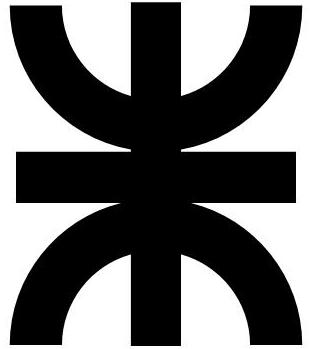
\includegraphics[height=20pt]{UTN_logo.jpg}}}
    \makecell[cl]{
        Universidad Tecnológica Nacional \\
        10 Noviembre Año 2025 %fecha 
    }}

\fancyhead[R]{\footnotesize
    \makecell[cr]{
        Técnicas Digitales III \\
        Daniele, Fernando %catedra y profesores
    }}

\fancyfoot[L]{\thepage}

\vspace{\fill}
{\huge \noindent \textbf{Desarrollo de un Sensor de Colores por Reflexión} \par} % title 

\vspace{1.5cm}
\noindent
\textbf{Beck, Federico}\\
Departamento de Ingeniería Electrónica,\\ Facultad Regional San Francisco, Córdoba, Argentina.\\
\href{mailto:federicobeck91@gmail.com}{federicobeck91@gmail.com}\par
\vspace{0.5cm}
\noindent
\textbf{Perez, Mariano}\\
Departamento de Ingeniería Electrónica,\\ Facultad Regional San Francisco, Córdoba, Argentina.\\
\href{mailto:perezmariano7401@gmail.com}{perezmariano7401@gmail.com}\par

\section{Introducción}
El color es una percepción visual que surge debido a la detección de diferentes longitudes de onda que no son absorbidas por un objeto o superficie. El conjunto de señales de distintas frecuencias compone el color de dicho objeto. Éstas, dentro del espectro visible de la luz, abarcan una gama de colores que va desde el rojo, con frecuencias más bajas y longitudes de onda más largas, hasta el violeta, con frecuencias más altas y longitudes de onda más cortas.

Durante el desarrollo de este trabajo, se diseñara e implementará un dispositivo que permita determinar el color de una superficie mediante la reflexión de luz.

El circuito utiliza LEDs RGB WS2812 como emisores, ya que cuentan con un factor de forma compacto, intensidad regulable, y un protocolo de comunicación sencillo. Además, se utilizan resistencias dependientes de la luz (LDR) con sus correspondientes circuito de adaptación de señal como receptores.

Debido a la baja trazabilidad de los LDR en general, y su amplio rango de respuesta (que va desde unos cuantos kilo-ohmios hasta el orden de los mega-ohmios), se implementará un procedimiento de calibración, que permitirá al dispositivo tener referencia de los valores medidos para superficies blancas y negras, con el objetivo de mejorar las mediciones obtenidas. Por esta misma razón, se utilizarán fuentes de corriente regulables que permitan mantener a las mediciones dentro del rango de tensiones aceptables para su lectura con el ADC del microcontrolador, que en el caso de la RP Pico es de \qtyrange{0}{3.3}{\V}.

El sensor consta de dos etapas, la primera esta compuesta por el conjunto emisor-detector y su circuito de acondicionamiento. El emisor es un LED RGB capaz de emitir luz roja, verde y azul por separado, la cual será reflejada sobre el objeto a medir e incidirá sobre el detector. El detector utilizado es una resistencia dependiente de la luz, la cual varía su resistencia dependiendo de la luz que incide sobre la misma. La variación de resistencia se debe convertir en una variación de tensión para que pueda ser procesada, para ello se utiliza una fuente de corriente constante.

La segunda etapa abarca el muestro y procesamiento de datos. Mediante el conversor analógico-digital (ADC) se muestrea la salida del circuito acondicionador luego de que la superficie a medir se ilumina. Las muestras son posteriormente filtradas de manera digital. Finalmente, los valores de tensión muestreados y filtrados se convierten en un valor entero de 8 bits, que representará la intensidad de luz reflejada. El proceso se repita para los tres colores RGB de forma secuencial.

Las mediciones se deben realizar aisladas de la luz ambiente, por lo que se utilizará una carcasa impresa en 3D para evitar que la luz ambiente interfiera en las mediciones y cause irregularidades.

La disposición de emisor y receptor se hará utilizando una configuración a \qty{45}{\degree}, tal como se muestra en la Fig. \ref{fig:montaje}. De esta manera se evita que la reflexión especular incida sobre el receptor, ya que esta no aporta información útil para las mediciones \cite{avago_rgb_color_sensing}, como si lo hace la reflexión difusa.

\begin{figure}
    \centering
    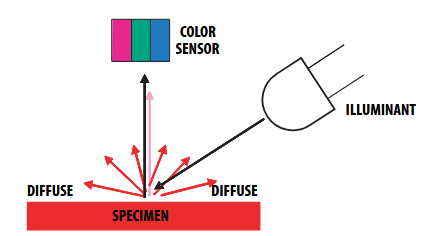
\includegraphics[width=0.5\linewidth]{img/montaje.png}
    \caption{Montaje de emisor y receptor.}
    \label{fig:montaje}
\end{figure}

Se eligió el microcontrolador Raspberry PI Pico W para su uso como controlador central. El mismo será el encargado de servir el panel de control que permitirá solicitar una medición y visualizar los resultados de las últimas mediciones en una pantalla.

En el circuito de la Fig. \ref{fig:diagrama} se muestra el diagrama de bloques del dispositivo, donde se pueden apreciar las principales partes que lo componen.

\begin{figure}
    \centering
    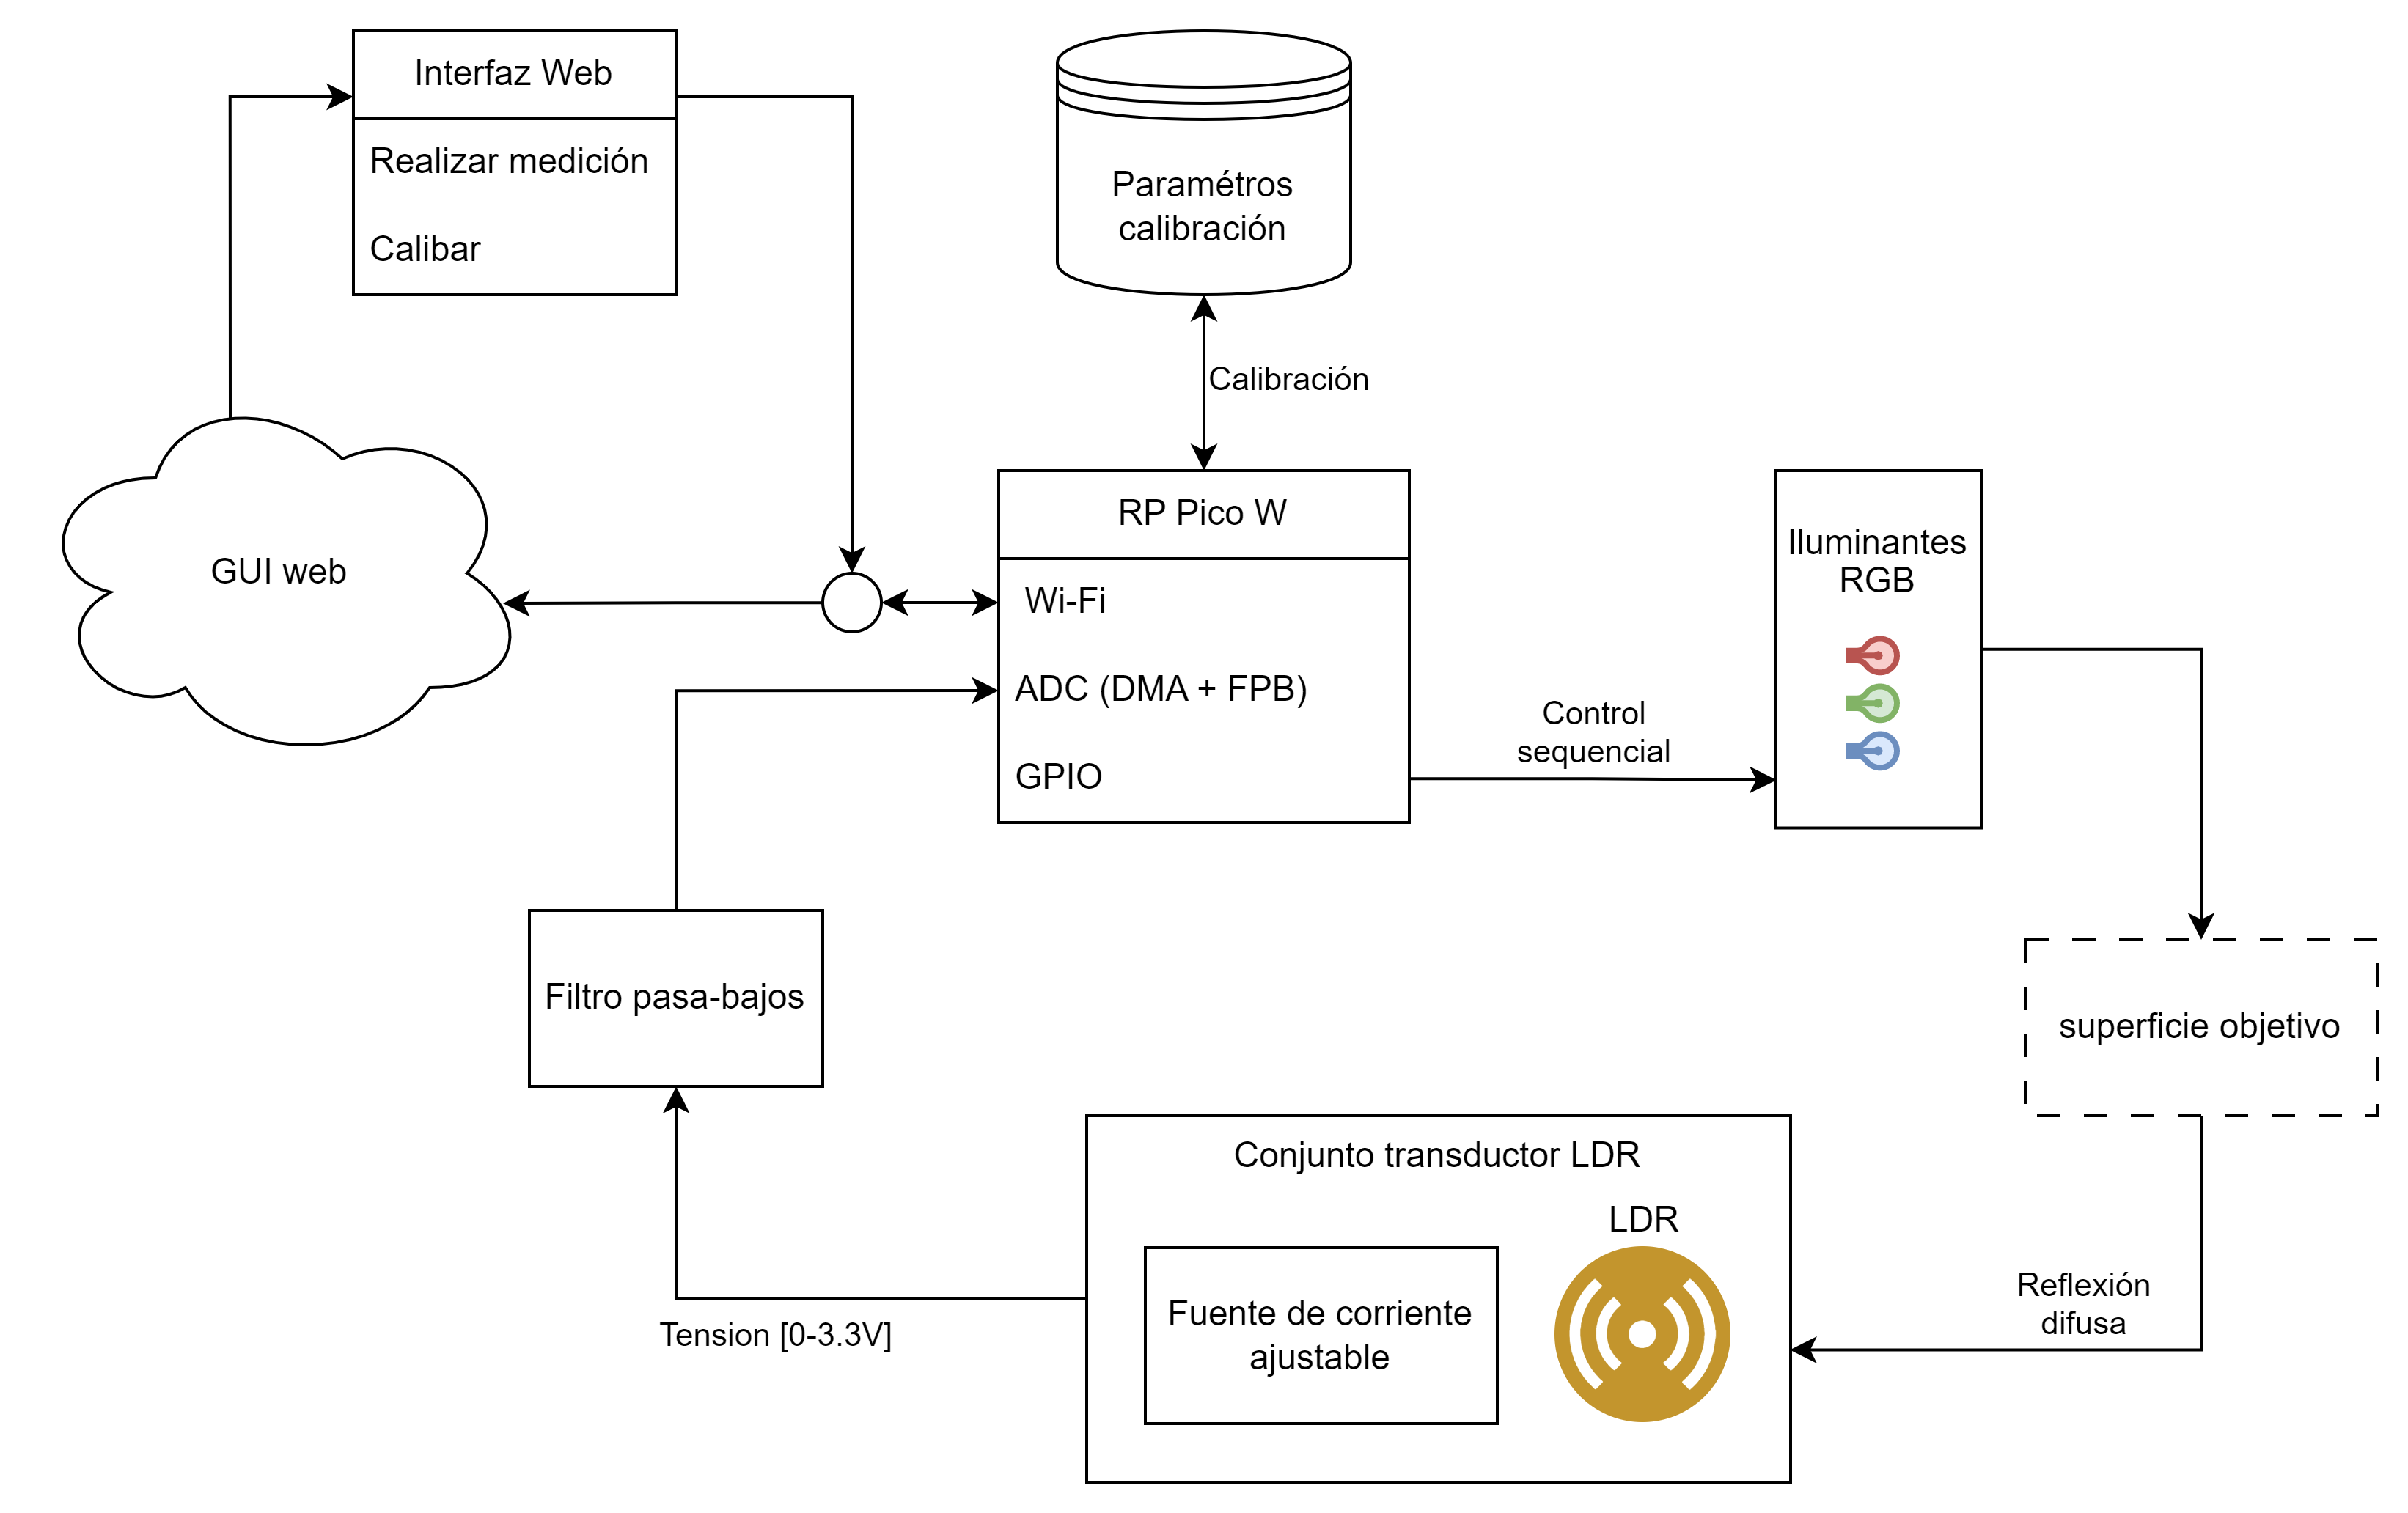
\includegraphics[width=0.9\linewidth]{img/diagrama_inicial.png}
    \caption{Diagrama de bloques preliminar del dispositivo.}
    \label{fig:diagrama}
\end{figure}

\subsection{Antecedentes}
Las opciones comerciales de este tipo de dispositivos suelen medir color al incidir sobre la superficie objetivo, rayos provenientes de una fuente de luz blanca. El color se determina mediante un arreglo de foto-detectores, que generalmente consisten de foto-diodos con filtros RGB; cada foto-diodo detecta la intensidad de luz reflejada para una longitud de onda especifica, y se determina el color de la superficie en base a las intensidades relativas de luz captadas por cada uno.

\subsection{Objetivos}
El objetivo de este trabajo consiste en desarrollar un dispositivo de bajo costo que permita determinar el color de un objeto con un grado de precisión aceptable mediante la reflexión de luz sobre su superficie. El mismo contará con un panel de control que permita visualizar los resultados obtenidos.


\subsection{Funcionamiento}
Como se observa en la Fig. \ref{fig:diagrama}, el sistema propuesto se basa en la implementación de una Raspberry Pi Pico W, encargada del procesamiento central. El proceso inicia con todos los LED apagados; transcurrido un tiempo determinado, se activa el LED rojo, que ilumina la superficie objetivo. Mediante un LDR se detecta la reflexión difusa de dicha superficie, y una fuente de corriente ajustable convierte la resistencia del sensor LDR en una señal de tensión. Esta señal analógica se pasa por un filtro pasa-bajos, con el fin de atenuar el ruido de alta frecuencia. Una vez filtrada, la señal es muestreada por el ADC de la Pico W, haciendo uso del DMA y se realiza un filtrado digital adicional para optimizar la adquisición de datos.

El procedimiento se repite de manera secuencial para los tres componentes de color (rojo, verde y azul), permitiendo obtener un conjunto de mediciones que representan la respuesta espectral de la superficie. Con estos valores, el sistema realiza el procesamiento y determinación del color resultante, el cual se visualiza a través de una página web. Dicha página también permite al usuario ejecutar mediciones de forma remota, calibrar el dispositivo y visualizar los resultados de mediciones previas. Todo esto se logra a través de un servidor web embebido dentro del microcontrolador.


\printbibliography

\end{document}


